\documentclass[lang=cn,12pt]{frbpaper}



\title{BUAA 冯如杯 \hologo{LaTeX} 模板(非官方)}
\subtitle{为专注写作而努力}
\author{\Large Pannenets.F \\  \Large{BUAA, SME}}
\date{\today}

\headofpaper{北京航空航天大学第三十届“冯如杯”学生学术科技作品竞赛参赛作品}


\begin{document}

\maketitle


\makeabstract

\section*{摘要}
以中国航空先驱冯如先生命名的北京航空航天大学“冯如杯”竞赛始创于1990年,是由学校科学技术研究院、教务处、学生处、科协、团委共同主办,科协、团委承办,在学校各学院党政领导的大力支持下开展的具有导向性、示范性和群众性并独具北航特色、彰显北航气韵、践行素质教育、弘扬创新精神的大学生学术科技活动。以“冯如杯”竞赛为标志的科技嘉年华于每年4-5月举办,以期周周有活动,场场有精彩,天天有创意。“冯如杯”竞赛积极引导广大学生开展创新实践与科学研究活动,培养学生自主创新能力,大力营造有利于青年学生健康成长和科技创新的良好氛围,对推进创新型校园的建设有着重大的战略意义。
\keywords{冯如杯, \hologo{XeLaTeX}, 论文模板}

\clearpage


\section*{Abstract}
With China aviation pioneer Mr Fung Joe guey named Beijing university of aeronautics and astronautics "fung Joe guey cup" contest was founded in 1990, is by the school, office, student affairs office, association for science and technology, science and technology research institute youth corps committee co-sponsored, association for science and technology, the youth corps committee to undertake, the school with the support from the party and government leadership and the colleges to carry out the guiding, demonstrativeness and mass character and unique characteristics, reveal buaa artistically buaa, practicing quality education and promote the innovation spirit of college students' academic science and technology activities. The Science and technology Carnival marked by the "Feng Ru Cup" competition is held every Year from April to May. "Feng Ru Cup" competition actively guides students to carry out innovative practice and scientific research activities, cultivates students' independent innovation ability, and vigorously creates a good atmosphere conducive to the healthy growth of young students and scientific and technological innovation, which is of great strategic significance for promoting the construction of innovative campus.
\ekeywords{Fengru's Cup, \hologo{XeLaTeX}, Paper Template}

\clearpage


\tableofcontents
\clearpage
\listoffigures
\clearpage
\listoftables
\clearpage



\makemain

\section{简介}

本模板完全依照基于第二十九届第三十届“冯如杯”学生学术科技作品竞赛论文撰写格式规范编写,两届规范并无不同,因此预计本模板可以用于之后的创意类、科技类、自然科学类的冯如杯论文写作。本项目的类文件编写很大程度上参考了 \href{https://github.com/ElegantLaTeX/ElegantPaper}{Elegant Paper} 项目的编写。本项目采用  BSD 3-Clause License .

\section{模块介绍}

本个章节用于介绍本模板的各个模块。

\subsection{字体}

本项目使用了方正字体,包含宋体、楷体、黑体、仿宋以及粗宋,以上字体可以在方正网站上下载使用,此外使用了微软自带的华文中宋、华文新魏,但是这两款字体不允许免费商用,因此请使用本模板的同学将本机自带的字体分别复制到  \lstinline{/fonts} 文件夹下的 \lstinline{HWXW.TTF} , \lstinline{HWZS.TTF} ,注意区分大小写。

\subsection{封面}

提供了 \lstinline{title} ,\lstinline{subtitle} ,\lstinline{author} \lstinline{date} 几个环境,均可以省略不填,以满足各种灵活的需求。其中作者项请通过 \lstinline{\Large} 等命令自行控制大小。如果需要使得时间精确到月,请使用 \lstinline{\frbtoday} 代替 \lstinline{\today}。

\subsection{摘要}

按照模板填写即可。

\subsection{图表}

在例章中提供了三线表格形式的 \lstinline{longtable} 环境以及对应的脚注,可以参考并修改。同时也可以自行使用 \lstinline{table} 等环境。

\subsection{公式与算法} 

数学公式环境:

\[\lim_{t \rightarrow \infty} \dfrac{\sin t}{t} = 0 \]

算法环境:

\begin{algorithm}
    \caption{遍历数组求最大值}
    \label{alg:array}
    \begin{algorithmic}
        \REQUIRE array \(a[m][n]\)
        \STATE \(init: i = 0, j = 0\)
        \STATE {\(ans \leftarrow a[i][j]\)} 
        \REPEAT 
        \REPEAT
        \STATE \(ans = \max (ans, a[i][j])\)
        \UNTIL{\(j = n\)} 
        \UNTIL{\(i = m\)}
    \end{algorithmic}
\end{algorithm}

\subsection{引用}

对于图、表与算法,提供了 \lstinline{\figref} ,\lstinline{\tabref} ,\lstinline{\algref} 可以得到形如 \figref{fig:test}, \tabref{sheet:ft}, \algref{alg:array} 的效果。
对于文献引用使用 \lstinline{\cite},这句话引用一些炼丹的论文 \cite{ghostnet,parashar2017scnn,park2017scale,abok},之后需要通过 \hologo{XeLaTeX} + \hologo{BibTeX}+ \hologo{XeLaTeX} * 2 ,生成完整的参考文献。


\begin{figure}[htb]\footnotesize
    \centering
    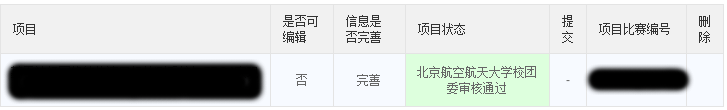
\includegraphics[width=0.5\textwidth]{figures/pass.png}
    \caption{测试}\label{fig:test}
    \label{fig:01}
\end{figure}



\begin{ThreePartTable}\footnotesize
    \begin{TableNotes}
        \item[a] 测试
        \item[b] 证明表格注释可用
    \end{TableNotes}
    \begin{longtable}{lll}\footnotesize\\
        \caption{傅里叶级数的奇偶对称性}\label{sheet:ft} \\ 
        \toprule    
        函数分类\tnote{a} & 三角级数性质\tnote{b} & 指数级数性质\\ 
        \midrule
        \endfirsthead
        % \toprule
        \multicolumn{3}{c}{\textbf{\tabref{sheet:ft}}~\textbf{续}}\\
        \toprule
        函数分类 & 三角级数性质 & 指数级数性质\\ 
        \midrule
        \endhead 
    
        \hline
        \multicolumn{3}{c}{见下页}\\   
        \bottomrule
        \endfoot
    
        \bottomrule
        \insertTableNotes
        \endlastfoot
        奇函数                                                                              & 只包含正弦函数分量                                                      & \(F(n \omega_1)\) 为纯虚数 相位谱只取\(\pm \dfrac{1}{2} \pi\) \\ 
        偶函数                                                                              & 只包含余弦函数分量                                                      & \(F(n \omega_1)\) 为实数 相位谱只取\(\pm  \pi\)             \\ 
        奇函数                                                                              & 只包含正弦函数分量                                                      & \(F(n \omega_1)\) 为纯虚数 相位谱只取\(\pm \dfrac{1}{2} \pi\) \\ 
        偶函数                                                                              & 只包含余弦函数分量                                                      & \(F(n \omega_1)\) 为实数 相位谱只取\(\pm  \pi\)             \\ 
        奇函数                                                                              & 只包含正弦函数分量                                                      & \(F(n \omega_1)\) 为纯虚数 相位谱只取\(\pm \dfrac{1}{2} \pi\) \\ 
        偶函数                                                                              & 只包含余弦函数分量                                                      & \(F(n \omega_1)\) 为实数 相位谱只取\(\pm  \pi\)             \\ 
    \end{longtable}
\end{ThreePartTable}

\subsection{致谢}

如果受到某些基金的支持,请在文末的致谢之后进行书写。

\subsection{附录}

如果没有需要,请把本文件末尾的\lstinline{\appendix} \lstinline{\addappheadtotoc} 注释掉。

\subsection{其他环境}

包括 Elegant Paper 提供的 定理、引理、命题、推论、定义、猜想、证明。对应在 \lstinline{.cls} 文件的 “定义中文环境” 一节。

\subsubsection{引理环境}


\begin{lemma}[一个引理]
    这可能是一个引理。
\end{lemma}


\subsubsection{定理环境}

\begin{theorem}[一个定理]
    这可能是一个定理。
\end{theorem}

\subsubsection{命题环境}

\begin{proposition}[一个命题]
    这是一个命题。
\end{proposition}

\section{使用方式}

本项目在 Manjaro Linux 以及 WSL-ArchLinux 平台的 TeXLive 2020 的测试,通过通过 \hologo{XeLaTeX} + \hologo{BibTeX} * 2 + \hologo{XeLaTeX},生成完整的参考文献论文。
或者 在命令行键入 \lstinline{latexmk -xelatex frb.tex}



\section{一个章节的例子}

这是一章专门用来测试各个章节层次是否可以正常工作的章节。

北航,一所有担当、有梦想、有情怀的大学。在这里中西文化汇通,科技与艺术交织,传承与创新共融,激情与灵感碰撞,在这里每一个舞台都可以绽放梦想,每一条道路都能够通向远方。六十余载办学薪火相传、硕果累累,这所中国年轻的重点高校——正焕发出勃勃生机,在建设扎根中国大地的世界一流大学的道路上砥砺前行。  


\subsection{节}

这是一节。

\subsubsection{小节}

这是一小节。


\section*{致谢}

本项目受到了 xxx 基金的支持。

\clearpage
\addcontentsline{toc}{section}{参考文献}

\bibliography{frbrefer}


\appendix
\addappheadtotoc

\end{document}